% begin module tangent-line-polynomial
\begin{frame}
\begin{example}[Tangent line to a polynomial]
Find an equation for the tangent line to the parabola $y = x^2 +2x + 1$ at the point $P = (\alertNoH{3,13}{2}, \alertNoH{6,12}{9})$.

\begin{columns}[c]
\column{.4\textwidth}
\psset{xunit=0.5cm, yunit=0.5cm}
\begin{pspicture}(-3.5,-0.5)(3.2,12.1)
\tiny
\fcAxesStandard{-3.2}{-0.5}{3.2}{12.1}
\fcXTickWithLabel{2}{$2$}
\fcYTickWithLabel{9}{$9$}
%Function formula: 1+2 (x)+(x)^{2}
\psplot[linecolor=red, plotpoints=1000]{-2.6}{2.44}{x 2 exp x 2 mul add 1 add }
\fcFullDot{2}{9}
\uncover<15->{
\psline[linecolor=blue](0.416666667,-0.5)(2.5,12)
\rput[l](1, 1){$y=6x-3$}
}
\rput[l](-3.3, 5) {\tiny$y=x^2+2x+1$}
\end{pspicture}
%\only<-7>{%
%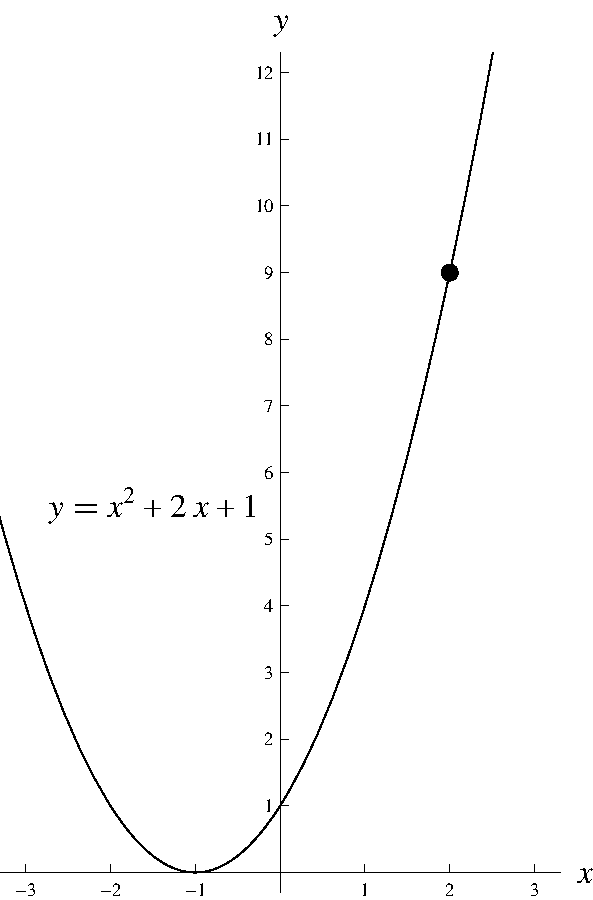
\includegraphics[width=4.0cm]{derivatives/pictures/tangent-line-polynomiala.pdf}%
%}%
%\only<8->{%
%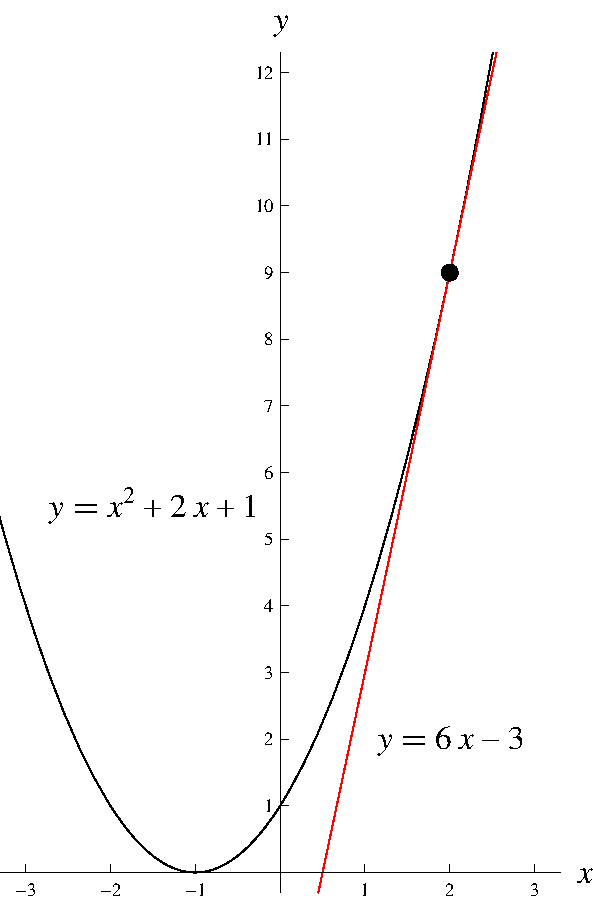
\includegraphics[width=4.0cm]{derivatives/pictures/tangent-line-polynomialb.pdf}%
%}%
\column{.6\textwidth}
\uncover<2->{%
Here \alert<handout:0| 2-3>{$a = \fcAnswer{3}{2}$} and $f(x) = x^2 + 2x +1$.
}%
\abovedisplayskip=0pt
\belowdisplayskip=0pt
\abovedisplayshortskip=0pt
\belowdisplayshortskip=0pt
\begin{align*}
\uncover<2->{\alertNoH{14}{m}} & \uncover<3->{ = }  %
\uncover<2->{\lim_{x\rightarrow \fcAnswer{3}{2}} \frac{\alertNoH{4}{f(x)}-\alertNoH{5,6}{f(\fcAnswer{3}{2})}}{x-\fcAnswer{3}{2}}}\\
& \uncover<4->{ = }  %
\uncover<4->{\lim_{x\rightarrow 2}\frac{ \alertNoH{4}{(x^2+ 2 x +\alertNoH{7}{1})} \alertNoH{7}{- \fcAnswerUncover{4}{6}{9}}}{x-2} }\\
& \uncover<7->{ = }  %
\uncover<7->{\lim_{x\rightarrow 2}\frac{\alertNoH{8,9}{ x^2+ 2 x \alertNoH{7}{- 8}}}{x-2}}\\
& \uncover<8->{ = }  %
\uncover<8->{\lim_{x\rightarrow 2}\frac{\fcCancel{10}{(\fcAnswer{9}{x - 2})}(\fcAnswer{9}{x+4})}{\fcCancel{10}{x-2}}}\\
& \uncover<10->{ = }  %
\uncover<10->{\lim_{x\rightarrow 2} (x+4)} \uncover<11->{\alertNoH{14}{= 6}.}\\
\end{align*}
\uncover<12->{
The tangent line: $y-\alertNoH{12}{9} = \alertNoH{14}{6}(x- \alertNoH{13}{2})$\alertNoH{15}{, or finally $y=6x-3$}.
}
\end{columns}
\end{example}
\end{frame}
% end module tangent-line-polynomial
